We have seen that replica selection flexibilities can render embeddings computationally hard.
We will now provide a more detailed look at this hardness result
and explore the minimal requirements for rendering replica selection hard.
In particular, we will show that already two replicas for each chunk type are sufficient to
introduce intractability.

Namely, we provide the NP-hardness results for two restricted variants of Virtual Cluster Embedding (Sections~\ref{ap:tworep-ma} and \ref{ap:tworep-ni}).
We augment the $\RS$ variant of $\VCEMB$ problem in the following way: by $\RS(k)$ we denote the problem where each chunk has the redundancy factor at most $k$.
In Section~\ref{ap:tworep-ma} we provide the hardness result for $\RS(2)+\MA+\FP$, and in Section~\ref{ap:tworep-ni} we provide the hardness result for $\RS(2)+\FP+\CC+\BW$.

Both problems are reduced from the problem $\TDPM$ (see Section~\ref{sec:3dm_intro} with no further restrictions.
The constructions are based upon the reduction of $\TDPM$ to $\FP+\RS+\MA$ (see Section~\ref{ssec:fprsma}) and the reduction of $\TDPM$ to $\FP+\RS+\CC$ (see Section~\ref{ssec:fprscc}).
However, in contrast to Section~\ref{ssec:fprscc}, in two replica variant without multiple assignment, we added the bandwidth constraints.
It is currently unknown to the authors of this very paper, whether the hardness result holds without bandwidth constraints (namely, whether the problem $\RS(2)+\FP+\CC$ is NP-hard).
The necessity for bandwidth constraints arises as to deal with restricted factor of replication, we need to introduce gadgets in the tree that makes the tree asymmetric.
Introducing bandwidth constraints allows to control the number of nodes spawning in certain parts of the tree.

\subsection{Two Replicas without Bandwidth Constraints}\label{ap:tworep-ma}

We now show that the 2-replica selection problem is even NP-hard
without capacity constraints.  In particular, we consider the problem
variant~$\RS(2)+\MA(4)+\FP$ with at most two replicas of each chunk type and assignment factor
four. There are no capacity constraints on links.

Our construction consists of two major modifications to hardness result without replication factor restrictions (for that result, refer to Section~\ref{ssec:fprsma}).

\textbf{Unique chunks on the comb.} First, we provide the tools for restricting the placement of nodes in certain parts of the tree.
In Section~\ref{ssec:fprsma}, due to symmetric structure of the tree, the carefully crafted threshold value allowed us to proof that e.g. no Triple Gadget ever had two or more nodes placed in it.
We still use the threshold value as the placement mechanism, but in this section, due to asymmetrical tree construction, we cope it with the concept of unique chunks on the comb (by the \emph{comb} we denote the balanced tree, where all non-root vertices has at most one child).

For the introduction to the concept of unique chunks, see the following example.
Suppose that within one $\VCEMB$ construction, we would like to encode not one $\TDPM$ instance, but two $\TDPM$ instances: $M_1$ and $M_2$, with disjoint universe and distinct number of triples to be chosen: $n_1$ and $n_2$.
We perform the following modifications to encoding provided in Section~\ref{ssec:fprsma}.
The multi-assignment factor grows by $1$, that is the instance we construct is the $\RS+\MA(4)+\FP$ instance.
We construct two subtrees $T_1$ and $T_2$, that correspond to resp. $M_1$ and $M_2$; we construct two two-edge-level combs $C_1$ and $C_2$, with number of leaves $n_1$, resp. $n_2$.
We attach $M_1$ and $C_1$ (resp. $M_2$ and $C_2$) to the common root and we name the resulting subtree the $P_1$, resp. $P_2$.
Next, we attach $P_1$ and $P_2$ to the common root.
In the end, the height of the tree grew by $2$.
Finally, we populate both combs with unique chunks, and we set the number of to-be-placed nodes to $n_1+n_2$.
We modify the threshold to be sum of the threshold for constructions for $M_1$ and $M_2$ plus $4\cdot (n_1 + n_2)$.
The last substrate of the threshold value corresponds to transportation of fourth chunk processed by each machine for the distance of four.

To see why the example indeed can solve two instances of $\TDPM$, we need the following observations.
First, we claim that no node is ever placed in a comb.
To prove this fact, we use the property of the comb that the leaves are highly separated, and the fact that each machine has to process $4$ chunks.
Next, we claim that the number of nodes spawned in $P_1$ (resp. $P_2$) is $n_1$ (resp. $n_2$).
To see this, consider any imbalance of number of spawned nodes; notice that some chunks in the underpopulated comb are processed outside of its $P_i$ subtree, resulting in the solution that exceeds the threshold.

\textbf{Families of chunk types.} The second tool that we introduce allows us to express the redundancy of chunks without actually replicating chunks more than two-fold.
For simplicity of introduction, we consider the scenario with multi-assignment factor of $1$.
For each chunk type $c$ with redundancy, we count the number of occurrences of replicas of such chunk in the tree, and name it $r_c$.
We replace the chunk type $c$ with $r$ chunk types, which we call the family $F_c$ of that chunk type.
For each occarrence of replica of $c$, we replace it with replica of any chunk type from the family (without repetitions).
To this point, the redundancy factor was reduced from $r_c$ to $1$.
Now, we construct the gadget $G_c$ for chunk type $c$, which consists of $r_c$ leaves, each hosting the second replica of each chunk type from family $F_c$.
We use the technique of unique chunks on the comb to constraint the number of nodes in $G_c$ to be exactly $r_c - 1$.
We provide necessary additional $r_c-1$ nodes to be placed.
Hence, exactly $1$ node is placed on chunk type of family $F_c$ outside the gadget $G_c$, and exactly $r_c-1$ nodes cover remaining $r_c-1$ chunk types inside gadget $G_c$.
All chunk types are processed, the replication factor was reduced to $2$, and the size of construction grew polynomially.

\textbf{Introduction to the reduction.} As we already stated, we modify the construction from Section~\ref{ssec:fprsma}.
As the way to deal with replication, we use the families of chunk types, which uses the unique chunks on the comb.
We extend the construction of a gadget for chunk type with redundancy, by incorporating the fact that the multi-assignment factor is $4$.
For the construction to remain correct with such multi-assignment factor, we introduce further chunks types with one chunk replica to place in the chunk gadget and use the excessive $3$ data processing capacities.

\textbf{Construction.}
For arbitrary instance~$I_{\TDPM}$ of~$\TDM$ we construct a~$\RS(2)+\MA(4)+\FP$ instance~$I_{\VCEMB}$ the way described in the remainder of this section.
Let $n = |X|=|Y|=|Z|$.
By $T$ we denote the set of all triples of $I_{\TDPM}$, and let $t = |T|$.
To access the elements of a triple $\tau \in T$, we introduce the following notation: $\tau = \langle e_X(\tau), e_Y(\tau), e_Z(\tau) \rangle$.
\maciek{are we using this notation?}
For each $e\in X\cup Y\cup Z$, by $T_e$ we denote the set of all triples that contain element $e$.
Let $\deg(e) = |T_e|$, and note that $\sum_e \deg(e) = 3\cdot t$.

We proceed with the construction as follows.

\paragraph{Chunk types and replicas}

We construct three types of chunks.
The first type corresponds to elements of the universe (that is, $X\cup Y\cup Z$).
The construction of such chunk types is similar to construction of chunk types in Section\ref{ssec:fprsma}, but to take into consideration the restricted replication factor, we construct the familiy of chunk types (as described in the introduction to this section).
Namely, for each element of universe $e$, we construct as many chunk types as there are occurences of $e$ in triples of $I_{\TDPM}$.
Each such chunk type has exactly two replicas.

The other two types are chunk types with one replica only, therefore called \emph{unique}.
We construct two types of unique chunks, distinguished by a different role in the construction.
For unique chunks we simply co-notate the chunk type with chunk replica.

Formally, the construction of chunk types and replicas unfolds as follows:
\begin{enumerate}
  \item For each triple $\tau \in T$, we construct $3$ chunk types, with two replicas each.
  We construct different chunk types for each triple $\tau$, which contain element $e$ (in total $\deg(e)$ chunk types).
  We refer to those replicas by $ch_1(e, \tau)$ and $ch_2(e, \tau)$.
  In total we construct $2\cdot \deg(e)$ chunk replicas.
  \item We construct~$n$ additional chunk types named
  ~$u_1, \ldots, u_n$ with one replica each.
  \item For each element~$e\in X\cup Y\cup Z$,
  we construct additional~$3\cdot(\deg(e) - 1)$ chunks, with one replica each.
  We call this set~$\UniqueE$.
\end{enumerate}

\paragraph{Tree}

We construct the tree that has the following structure (see Figure~\ref{fig:red-ma}):

\begin{figure}[t]
  \centering
  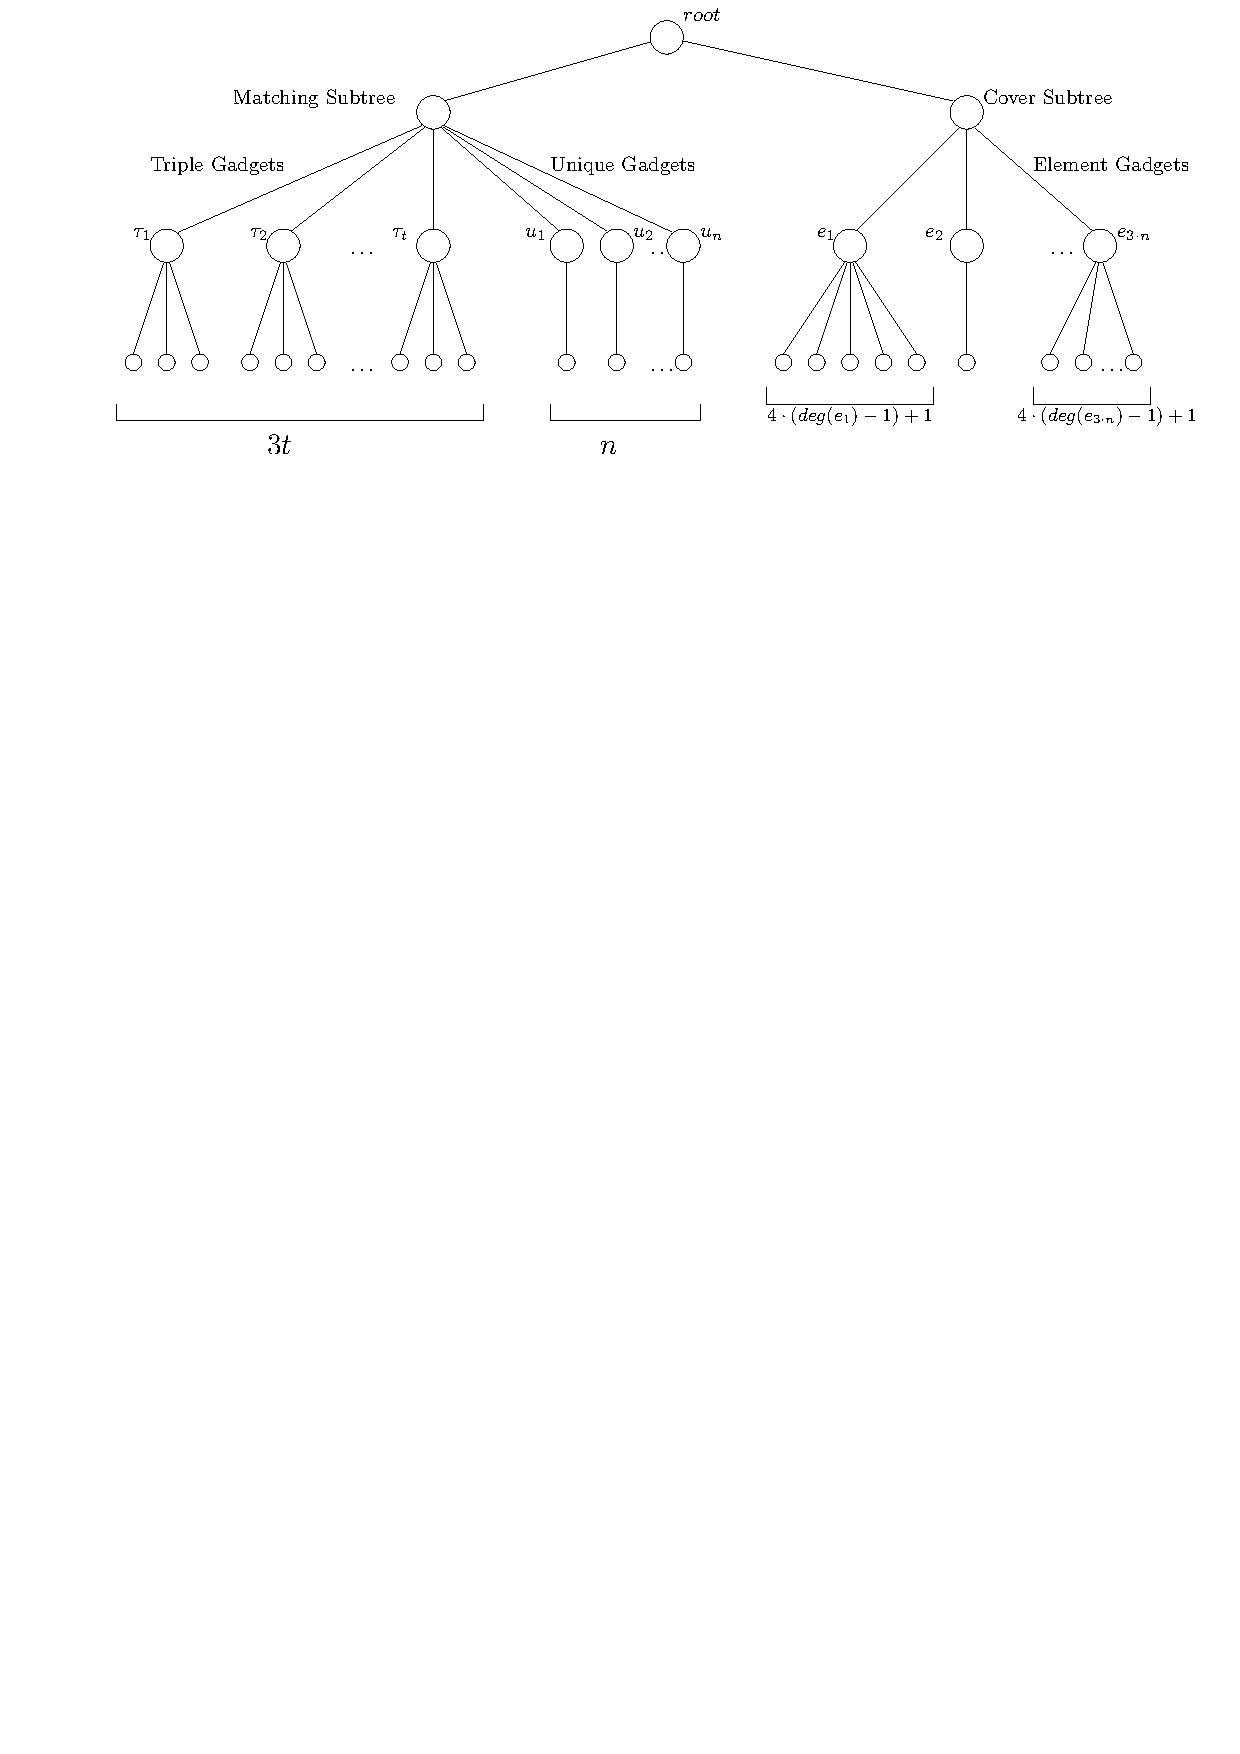
\includegraphics[width=0.99\columnwidth]{reduction/overview.pdf}
  \label{fig:red-ma}
  \vspace{-1em}
  \caption{Overview of the substrate network}
  \vspace{-1em}
\end{figure}
\maciek{TODO FIGURE: $3\cdot n$ elements instead of $n$}


\begin{enumerate}
  \item The physical network consists of two subtrees connected to the
  root: A {\MatchSubtree} and a {\CoverSubtree}. The
  {\MatchSubtree} consists of $t$ {\TripleGadgets}, one per each triple $\tau\in T$ and $n$
  {\UnqGadgets}. The {\CoverSubtree} consist of~$3\cdot n$ {\ElGadgets}, one for each element $e\in X\cup Y\cup Z$
  \item {\TripleGadget} consists of four vertices: three leaves and the root of the gadget.
  \item {\UnqGadget} consists of two vertices: the leaf and the root of the gadget.
  We construct the root node of the gadget not only to keep the tree balanced, but also to keep leaves of
  {\UnqGadgets} far from leaves of other \UnqGadgets. Note that \UnqGadgets{} form a comb.
  \item {\ElGadget} for element $e$ has a structure that depends on the number of triples that cover $e$. The {\ElGadget} consists of the
  root, and~$4\cdot(\deg(e)-1)+1$ leaves.
\end{enumerate}

\paragraph{Chunk Placement}
The chunks are placed as follows:
\begin{enumerate}
  \item \emph{Chunks in the Matching Subtree:} In {\TripleGadget} of triple $\tau$ we put
  three replicas:
 ~$ch_1(e_X(\tau), \tau), ch_1(e_Y(\tau), \tau), ch_1(e_Z(\tau), \tau)$, one per each leaf.
  \item \emph{Chunks in the Unique Subtree:} We place replicas
 ~$u_1,\ldots, u_n$ at the leaves of \UnqGadgets.
 \item \emph{Chunks in Element Gadgets:} Consider the \ElGadget{} for the element $e \in X\cup Y\cup Z$.
 We place two types of replicas in the leaves of the gadget.
 We put replicas $ch_2(\tau, e)$ for each $\tau \in T_e$.
 Additionally, we place all the replicas from set $\UniqueE$.
 In total, we place $4\cdot (\deg(e) - 1) + 1$ replicas, one per each leaf of the gadget.
\end{enumerate}

\paragraph{Other properties of the instance}
\begin{enumerate}
  \item \emph{Multiple assignment:} We set the multi-assignment factor to $4$.
  \item \emph{Number of nodes:} We allow to spawn
 %~$\numNodes = n + \sum_{e}(\deg(e)-1)$ nodes.
 ~$\numNodes = n + \sum_{e}(\deg(e)-1) = 3\cdot t - 2\cdot n$ nodes.
 \item \emph{Threshold:} We set the following threshold:
 %~$\Thr = 8\cdot n + 6\cdot\sum_{e}(\deg(e)-1)$
 ~$\Thr = 18\cdot t - 10\cdot n$.
 This value corresponds to the cost of solution, where $n$ nodes are matched to $4$ chunks that are in distance: $0, 2, 2$ and $4$ to the node, and remaining $|V|-n$ nodes are matched to $4$ chunks that are in distance: $0, 2, 2$ and $2$ to the node.
\end{enumerate}

\textbf{The reduction.}

Given any $\TDPM$ instance $I_{\TDPM}$, we produce corresponding instance of $\VCEMB$ variant, namely the $\RS(2)+\MA+\FP$ instance, in the way described above (in the construction paragraph\maciek{paragraph?}).
We refer to such $\RS(2)+\MA+\FP$ instance as the $I_{\VCEMB}$.

The reduction (Theorem~\ref{th:ma-reduction}) unfolds in two stages.
First, given a solution $S_{\TDPM}$ to $I_{\TDPM}$, we construct a solution $S_{\VCEMB}$ to $I_{\VCEMB}$.
This part is the easier of the two, and mainly consists of placing nodes in Triple Gadgets for triples chosen in $S_{\TDPM}$.

In the second stage, given $S_{\VCEMB}$, we construct the $S_{\TDPM}$.
In this stage, the main difficulty lies in showing that $S_{\VCEMB}$ has certain structure.

We call the {\TripleGadget} \textit{active}, if it contains a node at any leaf, and we call the node \textit{active} if it is placed in {\TripleGadget}.
Our goal is to show that in every feasible solution, exactly $n$ \TripleGadgets{} are active (Lemma~\ref{lem:n-active-ma}), and hence we can construct $S_{\TDPM}$ from the triples that correspond to active \TripleGadgets{} in $S_{\VCEMB}$.

In $I_{\VCEMB}$, chunks can be matched to nodes at distance $0, 2, 4$ or $6$.
  We call the matches at distance $0$ the \emph{free matches}, the matches at distance $2$ the \emph{neighbouring matches}.
  In addition we call the matches at distance $0$ or $2$ the \emph{short matches}, and the matches at distance $4$ or $6$ the \emph{long matches}.
  We call the distance between the pair of leaves the \emph{short distance}, if the distance between them is at most $2$, otherwise we call said distance the \emph{long distance}.

Proving the existance of more than $n$ long matches is sufficient to show that the instance is infeasible, as its cost exceeds the threshold.
To see this, note that the threshold value $\Thr$ corresponds to the cost of solution, where $n$ nodes has $1$ free match, $2$ neighbouring matches and $1$ long match at distance of $4$ hops, and remaining $|V|-n$ nodes has $1$ free match and $3$ neighbouring matches assigned.
Hence, at most $n$ long matches are present in any feasible solution.


\begin{lemma}
  In $S_{\VCEMB}$ there are have exactly $n$ nodes spawned in the \MatchSubtree.
  \label{lem:n-matchsubtree-ma}
\end{lemma}

\begin{proof}
 We claim that each node spawned in the \MatchSubtree{} results in at least one long match.
This fact is a consequence of the structure of the tree and the fact that multi-assignment factor is set to $4$.
For each node spawned in the \MatchSubtree{}, by the construction of the tree, the node has at most $3$ leaves in short distance, hence at least one of the matches is long.
Hence, we conclude that spawning more than $n$ nodes in the \MatchSubtree{} results in more than $n$ long matches, which results in infeasibility of the solution.
In addition, each node spawned in \UnqGadget{} results in at least $3$ long matches, as the only leaf in short distance is the leaf collocated with the node.

As at most $n$ nodes are spawned in \MatchSubtree{}, at least $|V|-n$ nodes are spawned in the \CoverSubtree.
Assume then that $|V|-n+i$ nodes spawned in the \CoverSubtree{} for non-negative $i$.
Now, we argue that such node configuration results in $3\cdot i$ long matches.
Consider the \ElGadget{} $g_e$ for element $e$.
The gadget $g_e$ has exactly $4\cdot(\deg(e)-1)+1$ leaves, each hosting exactly one chunk replica.
As $4\cdot(\deg(e)-1)+1 \mod 4 = 1$, spawnining $\deg(e)-1+j$ nodes in $g_e$ for non-negative $j$ results in at least $3\cdot j$ long matches by the fact that there are insufficient chunk replicas in the short distance.
Using the fact that $\sum_e(\deg(e)-1) = 3\cdot t - 3\cdot n = |V| - n$, by pidgeon-hole principle we conclude that indeed spawning $|V|-n+i$ nodes in the \CoverSubtree{} results in at least $3\cdot i$ long matches.

Consider the configuration with $|V|-n+i$ nodes spawned in the \CoverSubtree{}, and $n-i$ nodes spawned in the \MatchSubtree{}.
Such configuration results in at least $2\cdot i + n$ long matches, where $3\cdot i$ long matches come from the excessive nodes spawned in the \CoverSubtree{}, and $n-i$ long matches come from $n-i$ nodes in the \MatchSubtree{}.
Hence we deduce that $i = 0$, as otherwise the number of long matches would exceed $n$.

\end{proof}

\begin{lemma}
  In $S_{\VCEMB}$ no node spawned in \UnqGadget{}.
  \label{lem:no-unq-ma}
\end{lemma}
\begin{proof}
  By Lemma~\ref{lem:n-matchsubtree-ma}, exactly $n$ nodes spawned in the \MatchSubtree{}.
Suppose that out of $n$ nodes in the \MatchSubtree{}, a non-negative number of nodes $j$ spawned in the \UnqGadgets{}.
From the fact that each leaf of \UnqGadget{} has long distance to every other leaf, every node spawned in \UnqGadget{} result in at least $3$ long matches.
Hence, the total number of long matches is at least $n-j + 3\cdot j$.
Finally, for the solution to be feasible we allow at most $n$ long matches, therefore no node spawns in the \UnqGadget{}.
\end{proof}

\begin{lemma}
  In $S_{\VCEMB}$ there are have exactly $n$ active \TripleGadgets{}.
  \label{lem:n-active-ma}
\end{lemma}
\begin{proof}
  By Lemmas~\ref{lem:no-unq-ma} and \ref{lem:n-matchsubtree-ma} we conclude that $n$ nodes spawned in the \TripleGadgets.
As there are exactly $3$ replicas in each \TripleGadget{}, spawning more than one node in a single \TripleGadget{} results in at least additional $3$ long matches.
Hence, exactly $n$ \TripleGadgets{} are active.
\end{proof}

\begin{lemma}
  In $S_{\VCEMB}$ every chunk replica besides $u_1, \ldots, u_n$ is matched by a short match.
  \label{lem:short-ma}
\end{lemma}
\begin{proof}
  By Lemma~\ref{lem:n-active-ma}, exactly $n$ nodes are spawned in \TripleGadgets{}, and by Lemma~\ref{lem:no-unq-ma} we deduce that chunks $u_1, \ldots, u_n$ are matched by long matches.
  As at most $n$ long matches are allowed for the solution to be feasible, remaining matches are short.
\end{proof}

\begin{theorem}
  ~$\RS(2)+\MA+\FP$ is NP-hard.
  \label{th:ma-reduction}
\end{theorem}

\begin{proof}
  
  Let's take any instance $I_{\TDPM}$ of~$\TDPM$.
  We show that~$I_{\VCEMB}$ has a solution of cost~$\leq \Thr$ if and only if~$I_{\TDPM} \in \TDPM$ (there exists a perfect 3D matching in $I_{\TDPM}$).

  ($\Leftarrow$) Let's take any feasible solution~$S_{\TDPM}$ to $I_{\TDPM}$.
  We construct a solution~$S_{\VCEMB}$ in the following way:
  \begin{enumerate}
    \item We place~$n$ nodes in~$n$ {\TripleGadgets} (one per gadget) that correspond to triples in~$S_{\TDPM}$.
    The choice of exact leaf of the gadget to place a node is arbitrary.
    We match each such node to $3$ chunk replicas in the gadget it is placed, and we match $1$ arbitrary, unmatched chunk replica in {\UnqSubtree}.
    \item In each {\ElGadget} that corresponds to element~$e$, we place
   ~$\deg(e) - 1$ nodes and match them to arbitrary chunks in this
    gadget, which are not yet matched in any {\TripleGadget}.
  \end{enumerate}

  We can observe that every chunk type was processed, exactly $n + \sum_e(\deg(e) - 1)$ nodes are spawned, and each of the nodes process exactly $4$ chunk replicas.
  To see that indeed the produced solution do not exceed the threshold $\Thr$,
  we sum up the total transportation cost as follows.

  \maciek{This paragraph needs reformulation in terms of free, short and long}
  First, we focus on $n$ nodes that spawned in the Matching Subtree.
  Each of such nodes is collocated with one chunk replica that it is matched to,
  and it transports two chunk replicas from the same Triple Gadget, for each incurring the cost $2$.
  In addition, every such node process exactly one of chunks $u_i$, for each incurring the cost $4$.
  In total, each node spawned in the Matching Subtree incurrs the cost $8$.
  Next, we focus on the remaining $\sum_e(\deg(e)-1)$ nodes that are spawned in the Cover Subtree.
  Each such such node is collocated with one chunk replica it is matched to, and transports $3$ chunks, incurring the cost of $6$.
  Hence, the solution is indeed feasible.

  ($\Rightarrow$) Let's take any feasible solution~$S_{\VCEMB}$ to~$I_{\VCEMB}$.
  By Lemma~\ref{lem:n-active-ma}, exactly $n$ \TripleGadgets{} are active.
  We construct the solution $S_{\TDPM}$ from the set of triples that correspond to active \TripleGadgets{}.

  It remains to show that $S_{\TDPM}$ indeed matches every element of $X\cup Y\cup Z$.
  By Lemma~\ref{lem:short-ma}, each match of $ch(e, \tau)$ for each $e\in X\cup Y\cup Z$ and each $\tau \in T$ is matched by a short match.
  Hence, each active node~$v$ processes the 3 chunks that are placed in~$v$'s \TripleGadget.
  In each {\ElGadget} for element~$e$, one chunk $ch(e, \tau)$ for some $\tau \in T$ is not matched.
  Let's call this chunk instance~$\Unmatched(e)$, and let's call~$\Unmatched = \cup_e \Unmatched(e)$.
  Note that~$|\Unmatched| = n$.
  The set~$\Unmatched$ is covered by \ActiveNodes{}, and hence the set of triples in $S_{\TDPM}$ form a 3D Perfect Matching of $X\cup Y\cup Z$.
\end{proof}










\subsection{Two replicas without Multiple Assignment}\label{ap:tworep-ni}

\begin{enumerate}
  \item Two groups of nodes: for matching and for redundancy
\end{enumerate}